% overall design, architectural design, interface design, database design
% implementation - frontend (main, canvas, checklist) and backend (template creation, template storing, 3, 4)
% user diagram

% \section{Limitations}

% justify out of context wborkflow process

\section{Overall Design}
\label{design:overall}
% According to sections \ref{background:input_output}, and \ref{background:chens_design} in Background, we understood that a resource-based checklist generation tool could access to data models from each process in the workflow freely.

From section \ref{background:chens_design} in Background, we understood that the checklist generation tool contains three separable components: template creation, checklist template, and checklist usage. The \textbf{template creation} is the part in which a designer creates a \textbf{checklist template} for a specific process, and the \textbf{checklist usage} is the part where a workflow user comes and processes the \textbf{checklist template}.

According to sections \ref{background:workflowfm} and \ref{background:input_output} in Background, we also understood that we could access entities of each process through the execution engine as the resource of our checklist generation tool. After the completion of the checklist usage, the workflow will continue to the next process in the execution engine. With all the said, we drew the overall design diagram of how the checklist generation tool should work as well as be connected to the execution engine in Figure \ref{fig:overall_system_diagram} | we also provide a more detailed version in Appendix \ref{appendix:fig:overall_system_diagram}.

The figure starts at step 1 which the designer interacts with the tool to create a checklist template in the template creation. In the meantime, the workflow runs until it hits the process \#N, which requires the completion of the checklist. The workflow user needs to proceed with the checklist that the designer created in the checklist usage. After finishing the checklist, the workflow continues to the process \#(N + 1).


Due to the time constraints, we made the decision to focus on the template creation and the checklist template for this project and leave most features in the checklist usage for future work.

\begin{figure}[ht!]
    \centering
    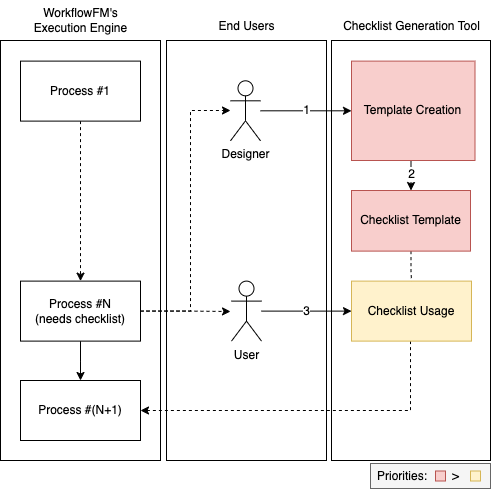
\includegraphics[width=0.65\textwidth]{overleaf/images/overall_system_diagram.png}
    \caption{Overall System Diagram}
    \label{fig:overall_system_diagram}
\end{figure}

\section{Functional Specification}
\label{functional_spec}
According to section \ref{background:chens_design} in Background and discussion with the product owner, we have concluded the functional specification into six functions and three original ideas from ourselves.

\begin{itemize}
    % \item \textbf{Template Creation}
    % \item \textbf{Template Saving}
    % \item \textbf{Checklist Viewing}
    % \item \textbf{Auto Generation*}
    % \item \textbf{Query Suggestion*}
    \item \textbf{Template Creation} is a function for a checklist designer to generate a new checklist template. Given the process details from WorkflowFM, the prototype should return a checklist template, which will be discussed more in section \ref{checklist_strcuture}.
    % \begin{itemize}
    %     \item Checklist's name is, as straight forward as it sounds, the name of this checklist template.
    %     \item Input information is the section that displays information from the values of the process's input data models.
    %     \item Form is the section where displays form components, including textboxes, calendars, dropdown menus, etc. Additionally, all output data models must be linked to every form components through dependencies linking.
    % \end{itemize}
    % This function is for the checklist designer to generate a new suggested template. Given a workflow process from WorkflowFM, the prototype should return a checklist template, which contains three sections: checklist name, input information, and output components.
    % explaining what this spec would do on the user's perspective
    \item \textbf{Input Information Query} is a function that allows a designer to add a new input information to the template. A checklist template allows the designer to add a new input information field to the template. A new input information field needs to be related to the original input information either as a foreign key or a parent key. A checklist template can use input information to query other input information to display in the section.
    % This function allows the designer to add a new input information to the template. A checklist template can use input information to query other input information to display in the section.
    \item \textbf{Form Adjustment} is a function that provides a designer with the flexibility to adjust components inside the form. There are five things a component can be adjusted: name, sequence order, requirability, visibility, and type.
    % Additionally, there are ten possible types of components: {tab}, {header}, {text box}, {paragraph}, {dropdown menus}, {choices}, {check boxes}, {date input}, {time input}, and {constant}.
    % things that can be adjust: type, required, hidden, order, name.
    % This function provides the flexibility to adjust a template to the checklist designer. A checklist template is able to add and adjust a new output component.
    \item \textbf{Dependencies Linking} is a function for a checklist designer to link the input and output dependencies to form components.
    \begin{itemize}
        \item An input dependency is a dependency that, when linked to a form component, causes that form component to connect to the value of the input data model.
        \item An output dependency is a dependency that, when linked to a form component, registers that form component as a component of the output data model.
    \end{itemize}
    % This function is for the checklist designer to link the input and output dependencies together.
    % An output component is able to link with the workflow process.
    \item \textbf{Template Saving} is a function that allows a checklist designer to save the template after finishing adjusting the checklist template.
    % This function is for the checklist designer to save the template after adjusting a checklist template.
    \item \textbf{Checklist Viewing} is a function that allows anyone to access a checklist template that has been created.
    % This function allows anyone to view the template that has been created.
    \item \textbf{Dependencies Validation} is one of the original functions specifically to validate dependencies in form components. It would give an error for every output dependency that is not linked to a form component.
    \item \textbf{Query Recommendation} is one of the original functions that provides an optional recommendation to a checklist designer to get suggested query information rather than manually inserting them one-by-one. The recommendation is based on the existing templates in the system.
    % This function provides the checklist designer an optional recommendation to get suggested query information rather than manually inserting one by one. The recommendation is based on the existing query information in the system.
    \item \textbf{Auto Generation} is one of the original functions that offers an optional automatic form generation on top of the template creation function for a checklist designer. This function automatically builds the whole template as well as links the dependencies based on the data models in from WorkflowFM.
    % This function offers an optional automatical dependency linkage for the checklist designer. The auto-link is based on existing, comparable templates from the system.
\end{itemize}

From the functional specification, we drew an use case diagram to visualise the connections between each function in Figure \ref{fig:use_case_diagram}. It is worth noting that some of the use case may not appear as a functionality in the functional specification, but they are generic enough to be in any system. We also provide sequence diagrams of each scenario in Appendix \ref{appendix:sequence_diagrams}.

\begin{figure}[ht!]
    \centering
    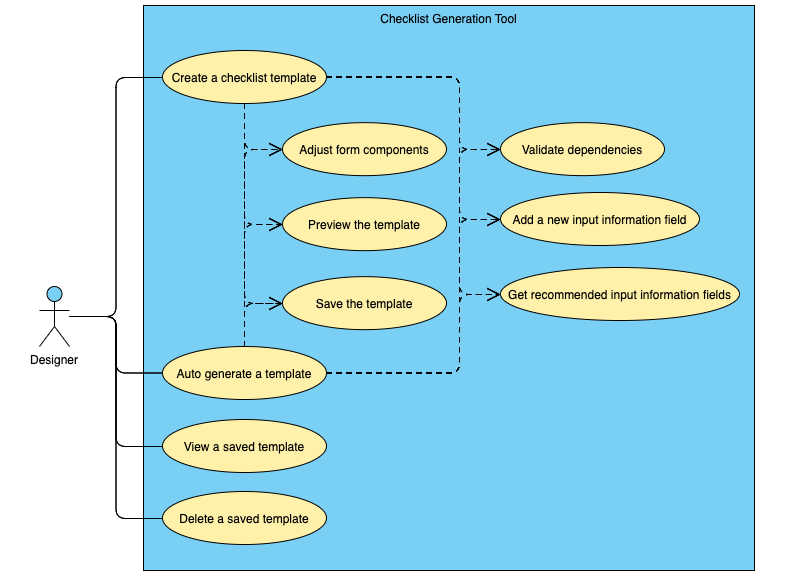
\includegraphics[width=0.8\textwidth]{overleaf/images/use_case_diagram.png}
    \caption{Use Case Diagram}
    \label{fig:use_case_diagram}
\end{figure}



\section{Software's Structure}
\label{design:software_structure}
According to section \ref{functional_spec}, we have grouped and categorised our project, as shown in Figure \ref{fig:software_structure}, into three parts: backend, frontend, and database.

\begin{figure}
    \centering
    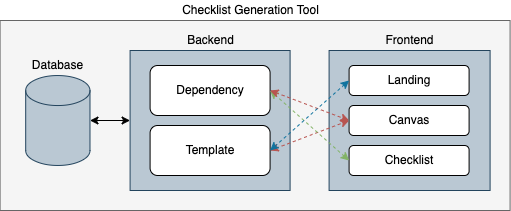
\includegraphics[width=0.7\textwidth]{overleaf/images/software_structure.png}
    \caption{Software's Structure}
    \label{fig:software_structure}
\end{figure}

\begin{itemize}
    \item Backend is the part which prepares and serves information from the database to the frontend. There are three routes as following:
    \begin{itemize}
        \item \textbf{Checklist} is the component that involves checklist-related features. This components only serves \textbf{Checklist Viewing} functionality.
        \item \textbf{Dependency} is the component involving all dependency-related features of the system. This contains \textbf{Input Information Query}, \textbf{Query Recommendation}, and \textbf{Auto Generation} functionalities.
        \item \textbf{Template} is the component involving all template-related features. This contains \textbf{Template Creation} and \textbf{Template Saving}. 
    \end{itemize}
    \item Frontend is an intermediate that allows both designers and workflow users to interact with the backend through web-based application interfaces. There are three main routes as following:
    \begin{itemize}
        \item \textbf{Landing} is the main page of the software. From this component, it could connect to other components in the software. This component connects to Backend's Checklist in order to display checklists' metadata.
        \item \textbf{Canvas} is the component that allows users to interact with the software to create templates from a workflow process. This part connects to both Backend's Dependency and Template in order to retrieve all information to facilitate users to build a template.
        % is the template creation screen. This screen connects to Backend's Denpendency and Template to create and save a template.
        Additionally, this part provides \textbf{Form Adjustment}, \textbf{Dependencies Linking}, and \textbf{Dependencies Validation}.
        \item \textbf{Checklist} is the component that allows people to view a saved checklist template. This component connects to Backend's Checklist to retrieve template's information.
        % is a screen that allows people to view a checklist template through its interface. This screen connects to Backend's Checklist to retrieve a saved checklist template's information.
    \end{itemize}
    \item Database is the storage of the system that stores the data models from WorkflowFM and details of created templates.
\end{itemize}

% Specifically for the screen \#4, we designed the input information and form sections to plan on what features we should be implementing, as seen in Figure \ref{fig:input_info_and_form}.
% This will be discussed more in Implementation.

% \begin{figure}
%     \centering
%     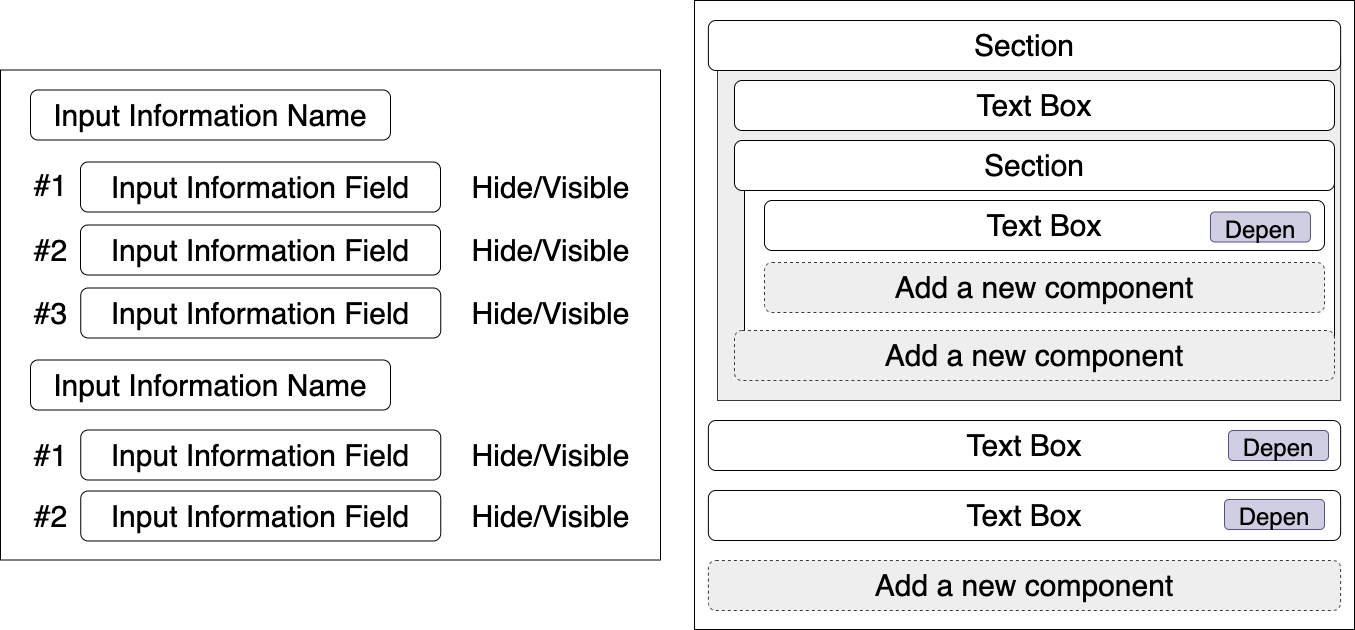
\includegraphics[width=0.9\textwidth]{overleaf/images/input_info_and_form.png}
%     \caption{Input Information's (Left) and Form's (Right) Interface Designs}
%     \label{fig:input_info_and_form}
% \end{figure}
\section{Checklist Template's Structure}
\label{checklist_strcuture}


\begin{figure}[ht!]
    \centering
    \textit{This example will be used to help explain the checklist} template's structure.
    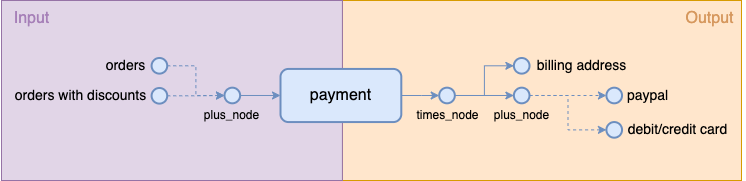
\includegraphics[width=\textwidth]{overleaf/images/template_example.png}
    \caption{Example Process}
    \label{fig:template_example}
\end{figure}

Given an example process in Figure \ref{fig:template_example}, we will assume this payment process needs a checklist for users to fill in billing address and either their debit/credit card information or their PayPal account. This process also has incoming input being either regular orders or orders with discounts.

We will assume that \verb!orders!, being an entity, contains two fields: order id and total price; \verb!orders with discounts! contains three fields: order id, total price, and discount code; \verb!billing address! contains two fields: home address and country; \verb!paypal! contains only paypal account; and \verb!debit/credit card! contains three fields: card number, expire date, and security code.




A checklist template is created by the template creation function. Its purpose is to perform a certain task for workflow users.
A checklist template contains three main parts: the name of the template, the input information, and the form components.

\begin{itemize}
    \item The name of the template is as straightforward as it sounds.
    \item Input information is the inputs' information that comes into the process.
    For example, in Figure \ref{fig:template_example}, the input information of this checklist template are the input part in the diagram: \verb!orders! and \verb!orders with discounts!. It is worth mentioning that being \verb!times! or \verb!plus! does not matter here. Every non-duplicate data model is counted towards input information.
    \item A form component is a representation of a form component, i.e. text boxes, calendars, dropdown menus, etc. For example, in Figure \ref{fig:template_example}, we could be six text boxes to cover everything (i.e. home address, country, paypal account, card number, expire date, and secuirty code).
    % \verb!paypal account!, \verb!debit/credit card number!, and \verb!security code!; and a date input for \verb!expire date!.
\end{itemize}

% As mentioned in Background section \ref{background:input_output}, the template creation only needs the name,  input, and output of the process to generate a checklist template. Thus, we consider all three of them as the template creation's input.
% For example, in Figure \ref{fig:template_example}, the template creation's inputs are shown in Table \ref{tab:process_input}.

% \begin{table}[ht!]
%     \small
%     \begin{tabularx}{\textwidth} { 
%         | p{\dimexpr.3\linewidth-2\tabcolsep-1.3333\arrayrulewidth}
%         | >{\centering\arraybackslash}X | }
%         \hline
%         \textbf{Process Name} & payment\\ 
%         \hline
%         \textbf{Inputs} & plus(orders, orders with discounts) \\
%         \hline
%         \textbf{Outputs} & times(billing address, plus(paypal, debit/credit card)) \\
%         \hline
%     \end{tabularx}
%     \caption{Template Creation's Inputs}
%     \label{tab:process_input}
% \end{table}

% We decided to use a tree data structure for checklist templates in order to. 
% The data models of checklist templates includes ChecklistTemplate, InputInformation, Details, and Component as shown in Figure \ref{fig:data_structure}.
% The checklist template, which is the output of the template creation, is also a repeated children structure (non-binary tree structure), similar to the input because we need to transform filled checklists to the tree structure and send them to the next process after the checklist usage. The input and output diagram is shown in Figure \ref{fig:system_input_output}.

% \begin{figure}[ht!]
%     \centering
%     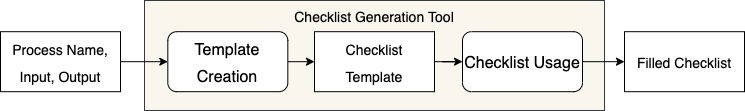
\includegraphics[width=0.8\textwidth]{overleaf/images/system_input_output.png}
%     \caption{System's Input and Output Diagram}
%     \label{fig:system_input_output}
% \end{figure}

% As stated in both \ref{intro:scope_of_work} and \ref{design:overall}, we only focus on the template creation. Thus, we only designed the data structure of the checklist template

We designed four models, as shown in Figure \ref{fig:data_models}, to represent the three main parts of a checklist template based on the functionalities in section \ref{functional_spec} and used these models across the system. Furthermore, the database was also designed based on these models, which the actual database design can be seen in Appendix \ref{fig:checklist_db_design}.
% Additionally, the relation between models and functions can be seen in Table \ref{tab:model_to_function}.
% Four models were designed to represent the three main parts of a checklist template as shown in Figure \ref{fig:data_models}.
\begin{itemize}
    \item ChecklistTemplate is a model representing the overall structure of a checklist template. It contains two other models inside: InputInformation and Component.
    \item InputInformation is a model representing the input information metadata of a checklist template, e.g. \verb!orders! and \verb!orders with discounts!. It contains Details model inside to the fields in the input information.
    \item Details represents a input information field under InputInformation. For example, order id and total price in \verb!orders!; and home address and country in \verb!billing address!.
    \item Component is model representing a form component in a template. For example, as shown in Figure \ref{fig:component_example}, we could have two root components which are sections. The first section is to represent the billing address, and the other one is to represent the payment methods (PayPal and card). Under the billing address section, it contains two text boxes of home address and country. Under the payment methods, it contains two more sections of PayPal and Card, which they contain fields inside.
    % is a tree-structured model representing a form component in a template. Additionally, it can recursively contain itself as children.
\end{itemize}


\begin{figure}[ht!]
    \centering
    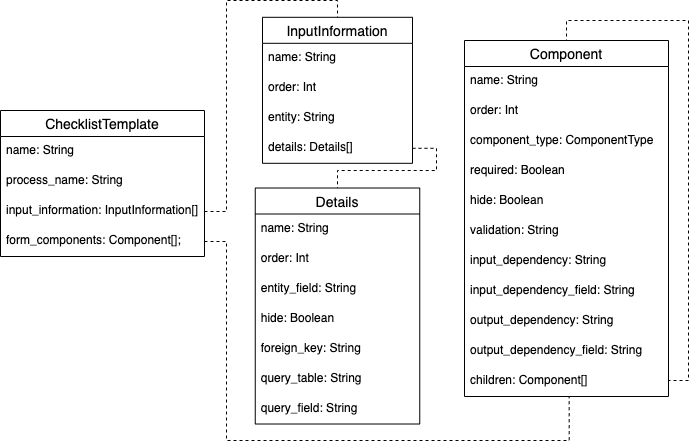
\includegraphics[width=0.9\textwidth]{overleaf/images/data_models.png}
    \caption{Checklist Template's Data Models}
    \label{fig:data_models}
\end{figure}

It is worth mentioning that the component model is a tree, similar to WorkflowFM's input and output. The rationale is for convenience for the auto generation function, which will be discussed in more detail in the Implementation chapter.

\begin{figure}[ht!]
    \centering
    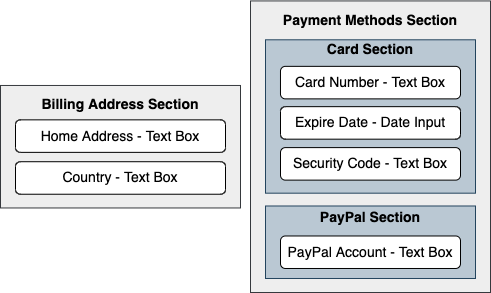
\includegraphics[width=0.6\textwidth]{overleaf/images/component_example.png}
    \caption{Example of Components}
    \label{fig:component_example}
\end{figure}

\section{Interface Design}
\label{interface_design}
We designed the interfaces of this project based on Chen's design \cite{checklistdesign} and popular form generators, such as Google Forms \cite{googleforms} and Microsoft Forms \cite{msforms}. We used Chen's design as the base design for the functionalities in the website and modernised the design based on the designs of popular platforms. The sketch of how each interface navigates is shown in Figure \ref{fig:overall_interface_design}.

\begin{figure}[ht!]
    \centering
    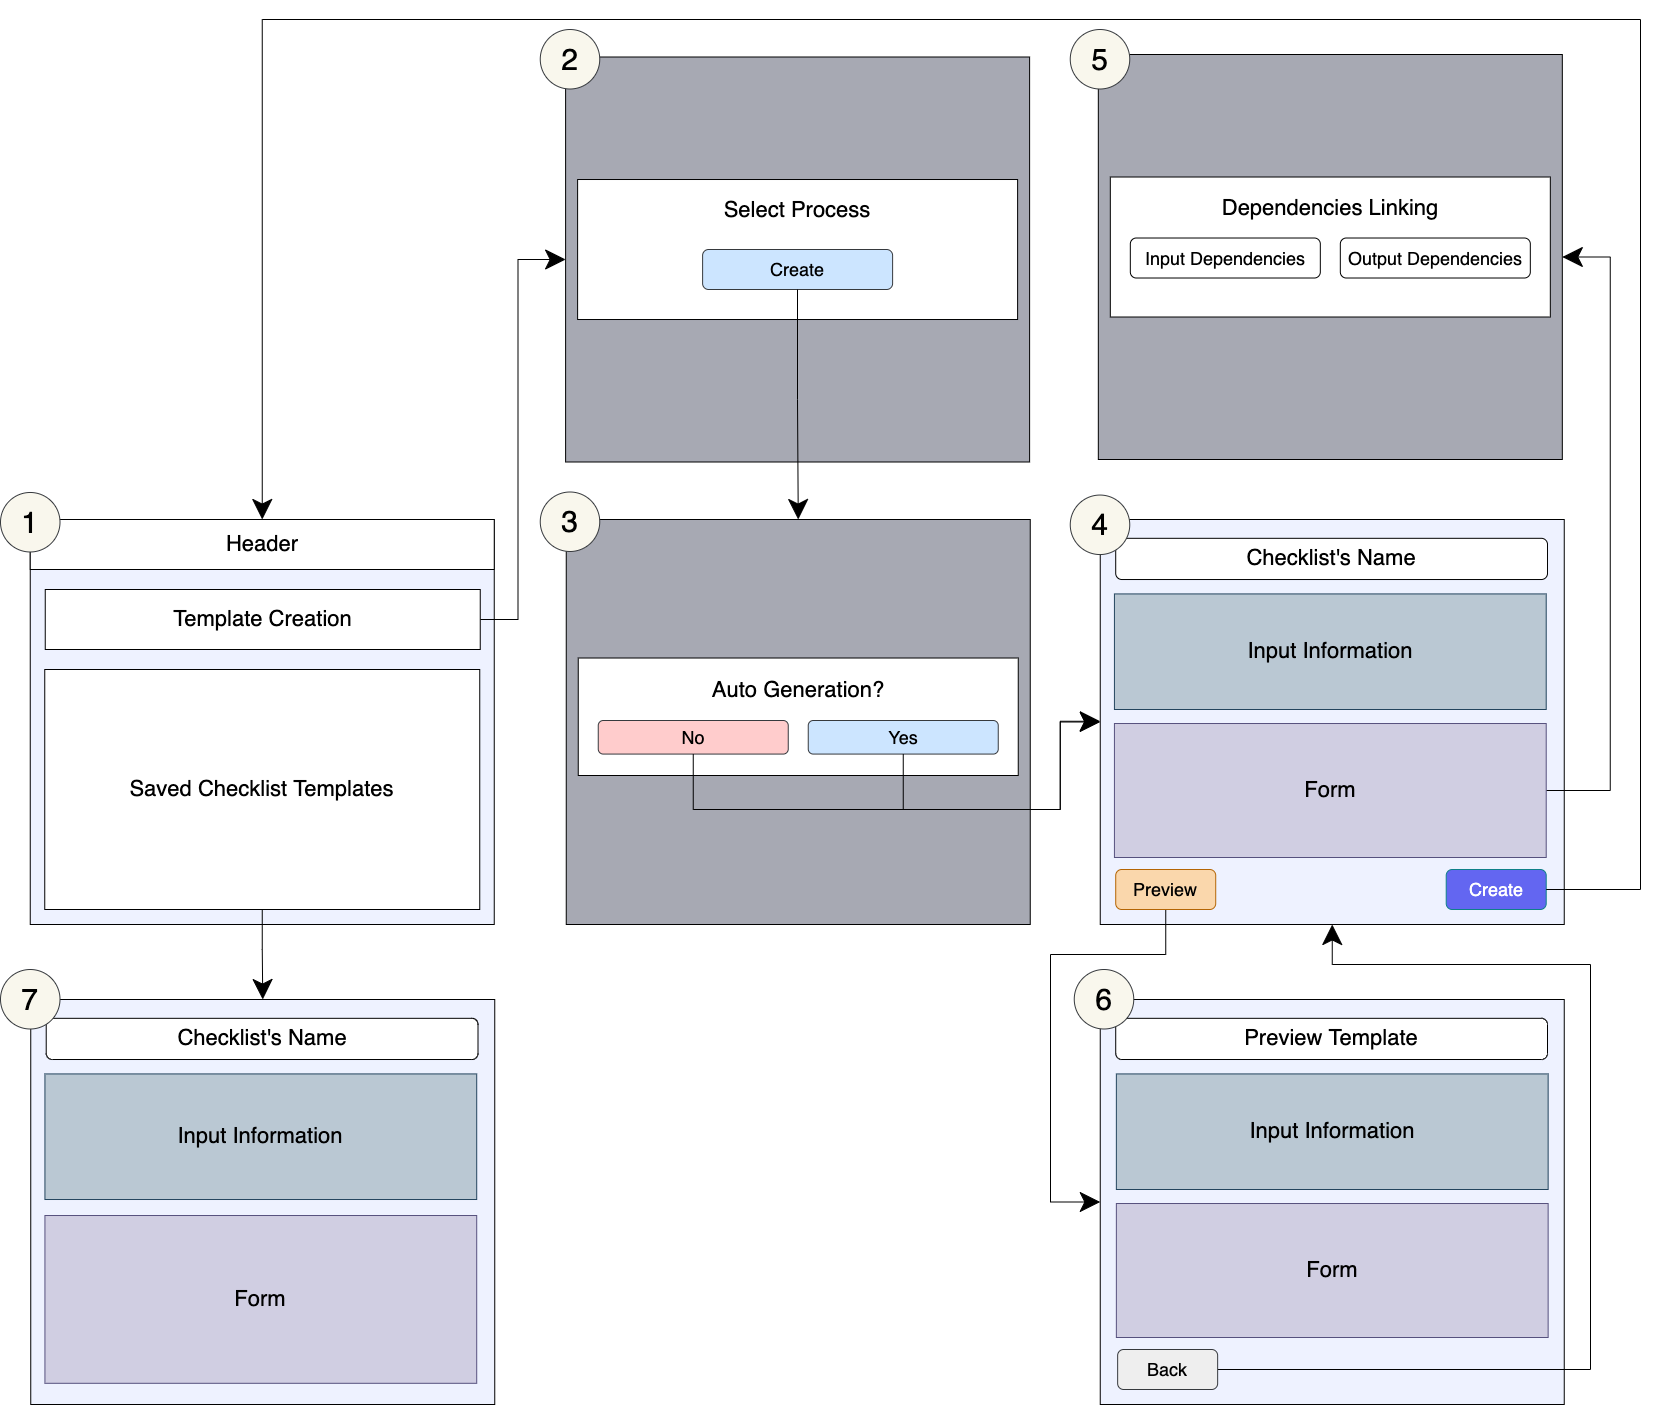
\includegraphics[width=\textwidth]{overleaf/images/overall_interface_design.png}
    \caption{Overall Interface Design}
    \label{fig:overall_interface_design}
\end{figure}

From the sketch, it can be seen that there are only three different screens (screens \#1, \#4, and \#8), one duplicated screens (screen \#6), and four popup screens (screens \#2, \#3, \#5, and \#7). Starting from screen \#1, this is the landing page (the main screen) that contains two sections: template creation and saved checklist templates. The template creation section will navigate users to screen \#2 to create a new template. Meanwhile, The saved templates section displays a list of saved templates in the system and will let users navigate to screen \#8 to view a saved template.

On screens \#2 and \#3, they are both popups that allow users to i) select a workflow process that users want to create a template for; and ii) select whether or not users want to use the template auto-generation to generate the template.

Screen \#4 is the canvas screen. This screen allows users to create or adjust the checklist template of the process that they select in screen \#2. There are three sections in this screen, including the checklist's name section, the input information section, and the form adjustment section. The details of each section will be explained in the Implementation chapter.
Screen \#4 can navigate to screen \#5 through the form section. Screen \#5 is a popup screen to manage dependencies for the dependencies linking function.

% Screen \#4 is the canvas screen. This screen allows users to create or adjust the checklist template of the process that they select in screen \#2. There are three sections in this screen, including the checklist's name section, the input information section, and the form section. The input information section consists of the name and fields of the input information, as shown in Figure \ref{fig:input_info_and_form} (Left). The form section consists of a group of components, as seen in Figure \ref{fig:input_info_and_form} (Right). A component can be one of the ten types: header, tab, textbox, paragraph, dropdown, choices, checkboxes, date, time, and constant. Additionally, header and tab components can contain a group of components.


Screen \#6 is a preview screen of the template that a user creates in screen \#4. It follows the same structure as screen \#4, but users are not allowed to adjust anything on this screen. Additionally, this screen has the same design as screen \#8. Users can navigate to this screen through the preview button and navigate back via the back button.

Users can save the template using the create button on screen \#4. This will navigate to a popup on screen \#7, which will eventually navigate back to screen \#1. After arriving on screen \#1, users should see the template they create displaying on the saved checklist templates section.

% From the sketch, it is obvious that there are only three different screens, one duplicated screen, and four popup screens. Starting from screen \#1, this is the landing page (the main screen) that contains two sections: template creation and saved checklist templates. The template creation section will navigate users to screen \#2 to create a new template. The saved templates section displays a list of saved templates in the system, and will let users navigate to screen \#8 to view a saved template.
% This screen contains three parts as follow to the checklist template's structure, which will be clarified more in section \ref{checklist_strcuture}.


% \begin{figure}[ht!]
%     \centering
%     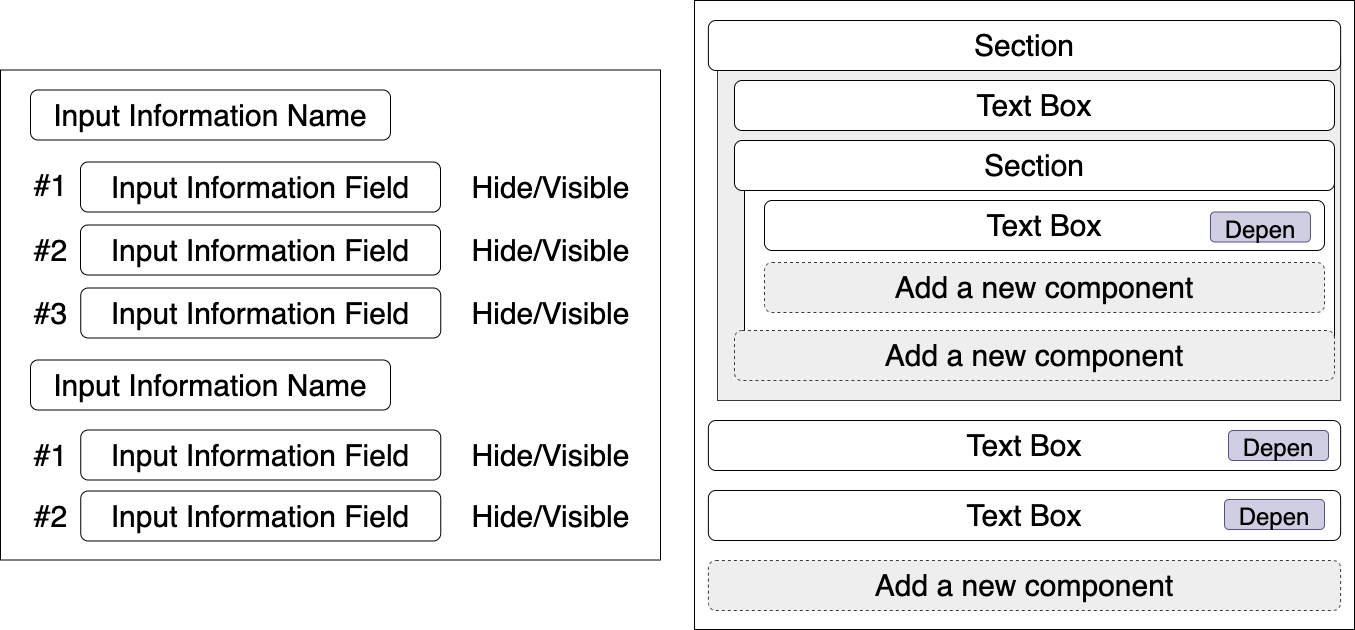
\includegraphics[width=0.65\textwidth]{overleaf/images/input_info_and_form.png}
%     \caption{Input Information's (Left) and Form's (Right) Interface Designs}
%     \label{fig:input_info_and_form}
% \end{figure}

% \section{Database Design}
% - main checklist design

% - templates, components

% - input\_information\_parent, input\_information\_child, input\_information\_child\_query





% \section{Use Case Diagram}



